%%% template.tex
%%%
%%% This LaTeX source document can be used as the basis for your technical
%%% paper or abstract. Regardless of the length of your document, the commands
%%% are all the same.
%%%
%%% The "\documentclass" command is the first command in your file. If you want to
%%% prepare a version of your article with line numbers - a "review" version -
%%% include the "review" parameter:
%%%    \documentclass[review]{acmsiggraph}
%%%

\documentclass[review]{acmsiggraph}

\usepackage{lineno}
\usepackage{float}
\usepackage{multirow}
\usepackage{array}
% \usepackage{units}
% \usepackage{color}

\usepackage{wrapfig}
\usepackage{tabulary}
\usepackage{amsmath} % assumes amsmath package installed
\usepackage{amssymb}  % assumes amsmath package installed
\usepackage{algorithm}
\usepackage[noend]{algpseudocode}



\algdef{SE}[DOWHILE]{Do}{doWhile}{\algorithmicdo}[1]{\algorithmicwhile\ #1}%


\newcommand{\todo}[1]{\textcolor{red}{TODO: #1}}

%%% Title of your article or abstract.

\title{Participatory Architectural Design and Fabrication with Natural Materials in Native Forms
}

\author{Hironori Yoshida\thanks{e-mail:hyoshida@hy-ma.com}   Takeo Igarashi\thanks{e-mail:takeo@acm.com}, Maria K Larsson, Masaaki Miki
 \\www.hy-ma.com, the University of Tokyo
}



\pdfauthor{Hironori Yoshida}

%%% Used by the ``review'' variation; the online ID will be printed on
%%% every page of the content.

\TOGonlineid{0542}

% User-generated keywords.

\keywords{Fabrication, Collaborative Design, Human-in-the-Loop}

% With the "\setcopyright" command the appropriate rights management text will be added
% to your document.

%\setcopyright{none}
%\setcopyright{acmcopyright}
%\setcopyright{acmlicensed}
\setcopyright{rightsretained}
%\setcopyright{usgov}
%\setcopyright{usgovmixed}
%\setcopyright{cagov}
%\setcopyright{cagovmixed}
%\setcopyright{rightsretained}

% The year of publication in the "\copyrightyear" command.

\copyrightyear{2016}

%%% Conference information, from the completed rights management form.
%%% The "\conferenceinfo" command has two parameters:
%%%    - conference name
%%%    - conference date and location
%%% The "\isbn" field includes the year and month after the article ISBN.

\conferenceinfo{SIGGRAPH 2016 Posters}{July 24-28, 2016, Anaheim, CA}
\isbn{978-1-4503-ABCD-E/16/07}
\doi{http://doi.acm.org/10.1145/9999997.9999999}

\begin{document}

%%% This is the ``teaser'' command, which puts an figure, centered, below
%%% the title and author information, and above the body of the content.

\teaser{
    \centerline{
       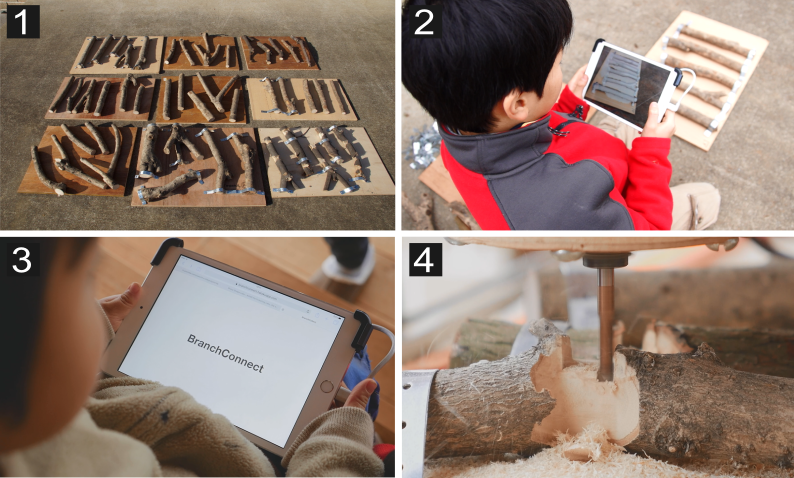
\includegraphics[height=0.23\paperheight]{images/fabrication/teaser1.png}
       \hspace{1mm}
         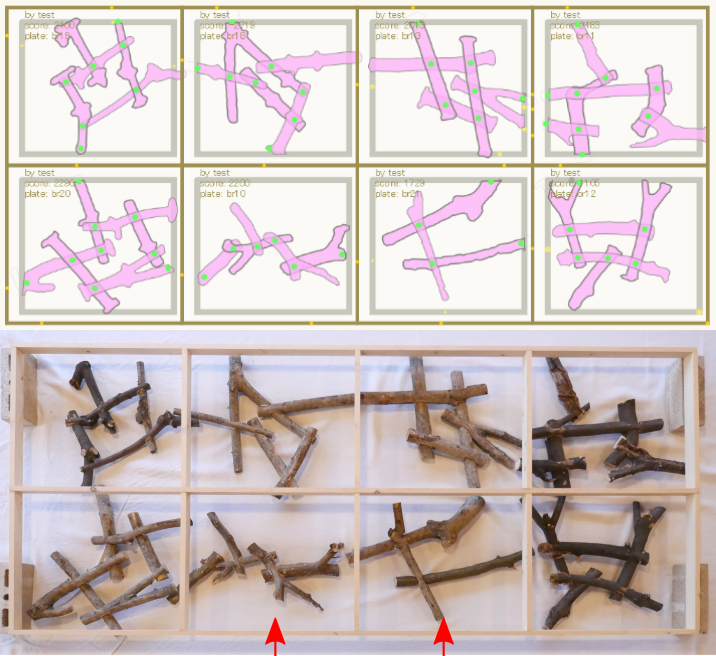
\includegraphics[height = 0.23\paperheight]{images/fabrication/teaser3.png}
 }
  \caption{Left: an overview of the workflow: 1. fix branches on plates. 2. scan the plates and upload the model. 3. play the game with scanned branches. 4. fabricate joineries by a CNC (Computer Numerical Control) router. Right top: branch layouts designed by authors and end users. 6 and 7 were fabricated in a workshop with participants. Right bottom: the fabricated 2D fence (2000 $mm$ $\times$ 900 $mm$). Each pair of branches is connected with rigid lapped joinery. }

  \label{fig:teaser}
}


\maketitle

\begin{abstract}
Diverse natural materials such as stones and woods have been used as architectural elements preserving their native forms since primitive shelters, however, the use of them in modern buildings is limited due to their irregular properties.
In this paper, we take the diversity as playful inputs for design task, and present our game-based design-fabrication platform for customized architectural elements.
Taking tree branches as a material in native forms, a game \textit{BranchConnect} enables end users to design 2D networks of branches and fabricate it by a CNC router.
The game considers fabrication constraints such as limitations with ordinal 3-axis CNC routers.
Each connection has a customized unique joint adapted to the native forms of branches.
The scoring system of the game guides users to design structurally sound solutions with given branches.
Together with low-cost mobile scanning devices, users with diverse contexts can contribute to design and fabrication process not only by playing the game, but also by collecting branches around their physical environments and uploading them to our online platform.
For validating our process, we conducted a workshop with children and their parents from a local community.
They collected branches in a nearby forest and contributed to design and fabricate a 2D fence with our system.
\end{abstract}

\linenumbers

%
% The code below should be generated by the tool at
% http://dl.acm.org/ccs.cfm
% Please copy and paste the code instead of the example below.
%
\begin{CCSXML}
<ccs2012>
<concept>
<concept_id>10010147.10010371.10010382</concept_id>
<concept_desc>Computing methodologies~Image manipulation</concept_desc>
<concept_significance>500</concept_significance>
</concept>
<concept>
<concept_id>10010147.10010371.10010382.10010236</concept_id>
<concept_desc>Computing methodologies~Computational photography</concept_desc>
<concept_significance>300</concept_significance>
</concept>
</ccs2012>
\end{CCSXML}

\ccsdesc[500]{Computing methodologies~Image manipulation}
\ccsdesc[300]{Computing methodologies~Computational photography}

\keywordlist

\conceptlist

\printcopyright

\section{Introduction}
Modern buildings are characterized by its uniformity; built upon the same principle of construction system consisting of standardized building components and its assembly process.
The standardized construction system is favored because of efficiency in design and production.
As a result, the structural performance of the whole building can be analyzed as each component and connection are standardized.
On the other hand, the excessive standardization induced similar styles of buildings which are criticized for being detached from local contexts ~\cite{frampton1983towards}, thus designers and architects actively use local materials preserving original forms as a catalyst of their design to the local context \cite{oliver1997encyclopedia}.
As the material is locally obtained, building represents and living get much closer, thus people using the building can easily commit design and fabrication, fostering the sense of belonging to the community \cite{weston2003materials}.
Traditionally, in case of constructing public and symbolic buildings, such as church, people in a community participated in fund raising or even in construction processes \cite{weston2003materials}.

Today, buildings with locally found materials are rare mainly because of economical issue.
As these materials are typically used by preserving their irregular properties, installation of them requires skilled craftsman for ensuring quality and structural validity, costing more than assembly of standard building parts and components.
 % can not compete with the efficiency of standardized systems.
Pye ~\shortcite{pye1968nature} argued craftsmanship as skills which can adapt its fabrication process according to irregular properties of materials and environments, and described as ``workmanship with risks'' in contrast to `workmanship with certainty''.
Since such a task require years of training thus it is difficult to be automated, the use of them is favored but limited in modern living environment, such as sculpture or other decorative works.
Also the knowledge to process natural materials are not explicit, thus users can not easily install such materials even though materials themselves are accessible.

%  thus the use of native forms typically inaccessible for end users and costs more than standardized construction system.
% Therefore, the use of natural materials is favored but there is no systematic use to overcome

This paper aims to make the above-mentioned qualities of materials in native forms more accessible for end users by leveraging digital technologies.
We use locally obtained branches as they are everywhere.
Usually public service maintain them by pruning, storing, and chipping or burning with some costs.
The size of branches (from 50 -300 $mm$ in diameter) is too small for furniture or other structural applications as building components.
It is a challenge for digital design and fabrication to utilize the diverse branches in meaningful ways.
Theoretically, the combination of low-cost scanning and digital fabrication machines can handle natural materials in diverse native forms.
The key challenge here is design.
A possible approach is optimization: minimize an energy function consisting of structural and fabrication costs.
This approach, however, is limited to particular design scenario with specific materials.
Furthermore, the concept of optimum solution is well suited to goals such as efficiency or low-cost, but these goals are not the qualities materials in natives forms can compete with standardized construction systems.
Instead, we take humans in our scan-design-fabricate workflow not only to solve the design problem, but also to provide an opportunity for people to participate in the workflow.

In this paper, we report our case study to design and fabricate an architectural element out of irregularly shaped branches, using our humans-in-the-loop system.
An online platform was developed so that users can post branches found at hand and design with them through the online game \textit{BranchConnect} \footnote{Please visit and play the game. \url{https://branchconnect.herokuapp.com/start}}.
The game system itself helps users to design feasible branch layouts and enable them to fabricate customized joints to connect them together without screws and adhesives.
The design of our joint extends the traditional orthogonal lap-joints to various angles within a range, freeing the diverse forms of woods from orthogonal connections.
Physically collected branches are digitally scanned and stored in a cloud database \textit{BranchCollect}, and offline application \textit{Branch Importer} analyzes forms of branches and upload them to the database.
The simple visual feedback and scoring system of the game guide users to feasible solutions, which are further inspected by an offline application \textit{G-Code\footnote{G-Code is the generic name for a control language for CNC machines.} Generator} for CNC milling process.
The game system and developed import/export applications are currently limited to branches, however, the principle of human-in-the-loop with design is applicable for other kinds of materials with diverse irregular forms.
We hope our method sheds lights on materials such as waste from demolition of buildings for various design applications.

In summary, our contributions are
\begin{itemize}
 \item{a workflow enabling to take natural materials in native forms as design components.}
 \item{an online game-based approach to participatory architectural design and fabrication.}
 \item{a method to design and fabricate customized non-orthogonal joints using high-resolution contours.}
\end{itemize}

\section{Related Work}
3D printers and CNC routers made digital fabrication more accessible, and pre-fabricated customized building components are often used in buildings nowadays \cite{knaack2012prefabricated}.
According to the theory by Pye \shortcite{pye1968nature}, these components are processed from highly standardized material, thus its digital fabrication process is ``workmanship with certainty''; a batch process of reading G-Code and strict execution of the code.
On the other hand, as ``workmanship with risks'' in digital fabrication, interactive fabrication enables machines to pick up uncertain happenings and react on it \cite{willis2011interactive}.
Mueller and her colleagues developed interactive laser cutting, taking user inputs and recognizing placed objects in a fabrication scene \cite{Mueller:2012:ICI:2380116.2380191}.
While their system interprets objects as simple platonic geometry, our work interacts with the native forms of irregularly shaped branches.
Crowdsourced Fabrication project took advantage of humans-in-the-loop in their fabrication system \cite{lafreniere2016crowdsourced}.
Similarly, an architecture-scale additive manufacturing with humans was built with guidance system \cite{Yoshida:2015:AHA:2809654.2766951}.
Unlike these works, our work puts emphasis on the involvement of humans in design.
As a crowdsourced design system, Talton and colleagues developed a platform for light users to design trees and plants \cite{talton2009exploratory}.
Our work also developed online collaborative design platform but directly linked to the real-world.

There are few works that take natural materials in native forms as design components.
Schindler and his colleagues used digitally scanned wood branches and used them for furniture and interior design elements \cite{schindler2014processing}.
Monier and colleagues virtually generated irregularly shaped branch-like components and explored designs of large scale structure ~\cite{monier2013use}.
Using larger shaped forked tree trunks, \textit{Wood Barn} project designed and fabricated custom joints to construct a truss-like structure \cite{woodbarn}.
\textit{Smart Scrap} project digitally measured lime stone leftover slates from a quarry and digitally generated assembly pattern of slates \cite{smartscrap}.
An automated pick-and-stack process was explored with stones with irregular shapes. \cite{Yoshida:2015:AHA:2809654.2766951}.
In industry, recognition of irregularly shaped objects is essential for waste management.
\textit{ZenRobotics} developed a system that sorts construction and demolition waste by picking objects on a conveyor belt using robotic hands \cite{lukka2014zenrobotics}.
For factory automation purpose, there is a system that recognizes irregularly shaped objects and sort them into a container \cite{sujan2000design}.
While these projects demonstrated the capability of digital fabrication processes to handle irregularly shaped materials, design process with native natural materials is still dependent on experts.

Cimerman discussed architectural design practices that took computer-mediated participatory (architectural) design \cite{cimerman2000participatory}.
He mentioned three motivations of digital participatory design: 
1. including stakeholders in creation of one's environment. 
2. experimenting diverse design tastes from multiple point of views.
3. solving complex design tasks with full of diverse solutions.

Database of available local materials allows people with various backgrounds to involve in design process, which could lower the design cost with natural materials in native forms.
We took inspiration from existing gamification systems.
For example, \textit{Nano-Doc} took gamification approach to search valid nano-particle designs against tumors out of infinite design space \cite{hauertcrowdsourcing}.
\textit{DrawAFriend} has developed an online game to collect big-data for drawing applications which assist humans with auto-stroke assistance \cite{limpaecher2013real}.
While these works developed games for collecting valuable data for solving medical or engineering problems, our game is served as a collaborative design platform, aiming to solve the socio-cultural issues in modern buildings such as generic design and detached context.

\section{Workflow}
As shown in Figure \ref{fig:teaser} left, our workflow starts from physically collecting branches.
In this section, we introduce two steps in the workflow shown in \ref{fig:teaser} left: Collecting and Scanning Branches (1 amd 2 in Figure~\ref{fig:teaser} left) and Fabrication (4 in Figure~\ref{fig:teaser} left).
As for the game (3 in Figure~\ref{fig:teaser} left), please refer Section \ref{sec:game}.
The collected branches are uploaded to cloud database by \textit{Branch Importer}, and served to the online game-based design application \textit{BranchConnect}.
The game system uses skeletons for its joint detection process, which works on browsers on laptop computers or mobile touch devices.
As shown in Figure \ref{fig:teaser} right, users can explore a global design with various layouts designed by multiple users.
Once layouts are selected the global design is fixed, these layouts are further inspected by \textit{G-Code Generator}, which generates customized joints for CNC milling.
After finishing the milling process, users physically assemble branches and complete the fabrication process.
The pipeline of the workflow is illustrated in the Figure \ref{fig:pipeline}.

\begin{figure}[ht]
  \begin{center}
    \includegraphics[width = 0.4\paperwidth]{images/workflow/pipeline.png}
    \caption{A pipeline from model acquisition to fabrication.}
    \label{fig:pipeline}
  \end{center}
\end{figure}

\subsection{Collecting and Scanning Branches}
Users can collect branches and upload to the online database.
Considering the mechanical constraints of CNC milling machine, branches are cut in certain length.
Please refer Section~\ref{sec:casestudy} for details.
The cut branches need to be firmly fixed to plates for milling process.
We use metal fixtures to attach them on a plate (See Figure~\ref{fig:skeleton}).
After attaching branches on plates, users can start scanning and acquire textured mesh model.
We describe the scanning setup further in details in Section~\ref{sec:casestudy}.

%As complete mesh model provides more robust results with 3D shapes of branches, we describe our process based on mesh model as an input.
Taking mesh model with colored texture, our \textit{Branch Importer} provides functions such as object detection, skeleton extraction, branch type classification, and fixture point setting.
The scanned result is a mesh model representing branches with a base plate.
The system first identifies branches by applying simple height threshold, and then applies contour detection.
The obtained 2D contours are used for extracting skeletons and clustering vertices in the mesh model.
Contours are triangulated and skeleton points are extracted from middle points on edges of triangles.
These middle points are compared with top view image.
If the point is inside of a contour, the middle point is counted as a skeleton point.
After extracting skeleton points, the connectivity of skeletons is analyzed.
In case grafting branch (Y-shaped branch) is detected, a new skeleton sub-branch is added.
The result is shown in Figure ~\ref{fig:skeleton}.
%Evaluating the number of sub-branches, the branch is morphologically classified.
Metal fixture locations are confirmed by simple mouse-clicks and marked as invalid, meaning that joints should not be placed on these points.
The acquired information is stored in a cloud database.

\begin{figure}[ht]
  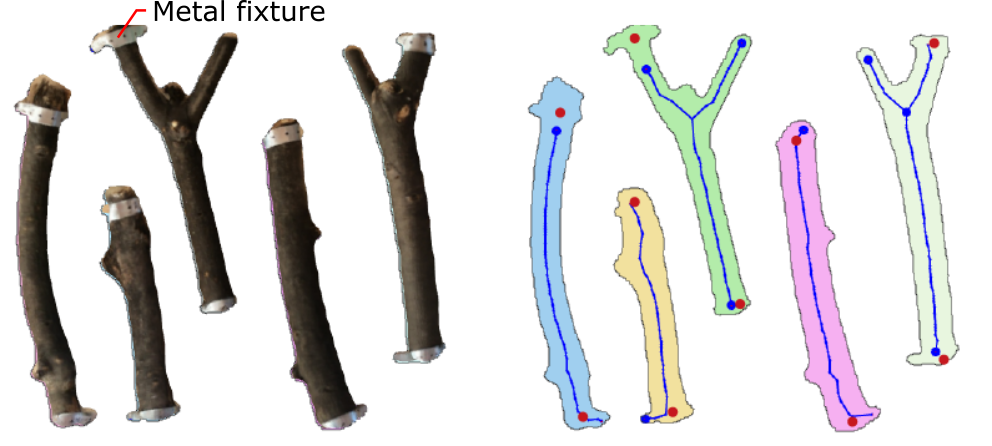
\includegraphics[width = 0.4\paperwidth]{images/importer/importer_2.png}
  \caption{An interface of \textit{Branch Importer}. Left: a top ortho-view image of textured mesh model. Right: Extracted skeletons are shown with blue dots. The beginning of skeletons is shown bigger dots, and the red dots are invalid points defined by a user. }
  \label{fig:skeleton}
\end{figure}


\subsection{Fabrication}
\label{sec:fabrication}
After a design is selected for fabrication, fabricatability of the design is further inspected by a high-resolution model.
The \textit{G-Code Generator} displays joints and milling paths on scanned orientations.
If it identifies an invalid joint in the high resolution model, a layout can be easily modified with simple mouse inputs (Figure \ref{fig:joint_geometry}.1 and \ref{fig:joint_geometry}.2).
Users can also change milling parameters such as offset ratio of milling paths, milling bit diameter, depth of joints, cutting speed, moving height and so forth.
After confirming the fabrication settings and milling paths, it generates G-Code.\\

Some fabrication factors such as invalid points due to metal fixtures and flipped (further described in Section \ref{sec:joint}) are already considered by \textit{Branch Importer} and the game system respectively.
Here, we describe the process to calculate joint geometry for fabrication.
The \textit{G-Code Generator} searches a set of four closest points on high-resolution contours (Figure \ref{fig:joint_geometry}.1).
By trimming contours of each branch at the corner points, we get \textit{side cuts} and \textit{center cuts} (Figure \ref{fig:joint_geometry}.4).
% Please refer Appendix~\ref{sec:sidecut} for details of this process.
\textit{Side cuts} have wedged corners for smooth assembly process.
The depth of the \textit{center cuts} is half of the top height at the joint position from a mesh model (Figure \ref{fig:joint_geometry}.4).
The bottom height is usually the height of the base plate, however, in case of under-cuts with incomplete mesh model, we calculate a half of the diameter from the 2D contour and subtract it from the top height.
The resulting geometry creates rigid joints with irregularly shaped sections.

\begin{figure}[h]
	\begin{center}
		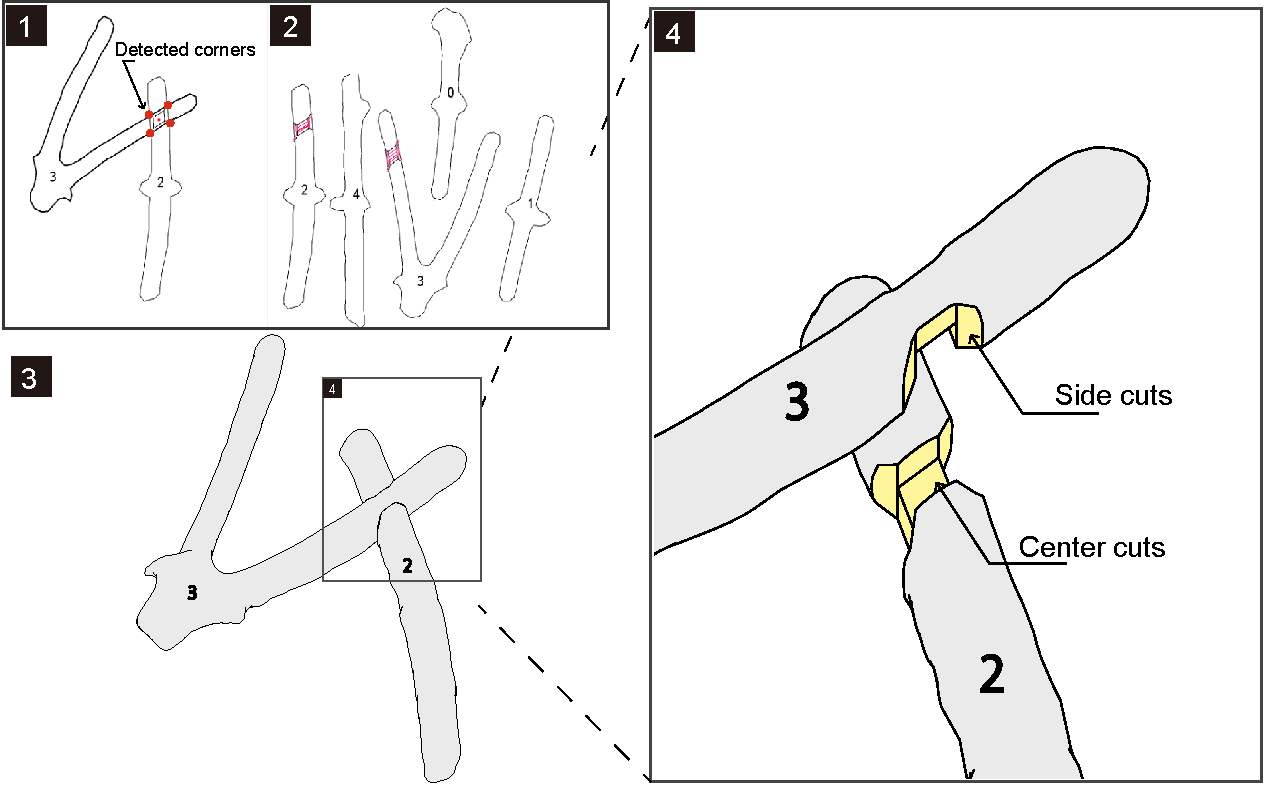
\includegraphics[width = 0.4\paperwidth]{images/system/joint_diagram.pdf}
		\caption{1, 2: an interface of G-Code Generator. 1. a layout defined by a user. 2. the original orientations of branches with generated milling paths with red color. 3. an assembled pair of branches with branch 3 is flipped. 4. milled branches with center cuts and side cuts.}
		\label{fig:joint_geometry}
	\end{center}
\end{figure}

\section{BranchConnect: The Game}
\label{sec:game}
The online game is accessible by laptops and mobile touch devices, and many users can play at the same time.
The objective of the game is to collect valid layouts of branches which are fabricatable with 3 axis CNC milling machines.
By analyzing the connectivity of branches and target points, the game informs the feasibility of a given layout.
Similar to our game, the work \textit{guidance system during furniture design} inspected connectivity, durability, and stability \cite{umetani2012guided}.
Unlike their work, our game puts emphasis on \textit{fabricatability}, as well as \textit{geometric connectivity}, and does not calculate structural performance of each joint.
%Instead, we limit valid layout space by selected joint conditions, and group conditions.
Instead we use simple geometric analysis to compute validity.
We also assume that every fabricated joint works as a rigid joint, thus single connection is counted as stable to hold a pair of branches.


%The workflow of the game is illustrated in Figure~\ref{fig:game_flowchart}.
%\begin{figure}[ht]
%  \begin{center}
%    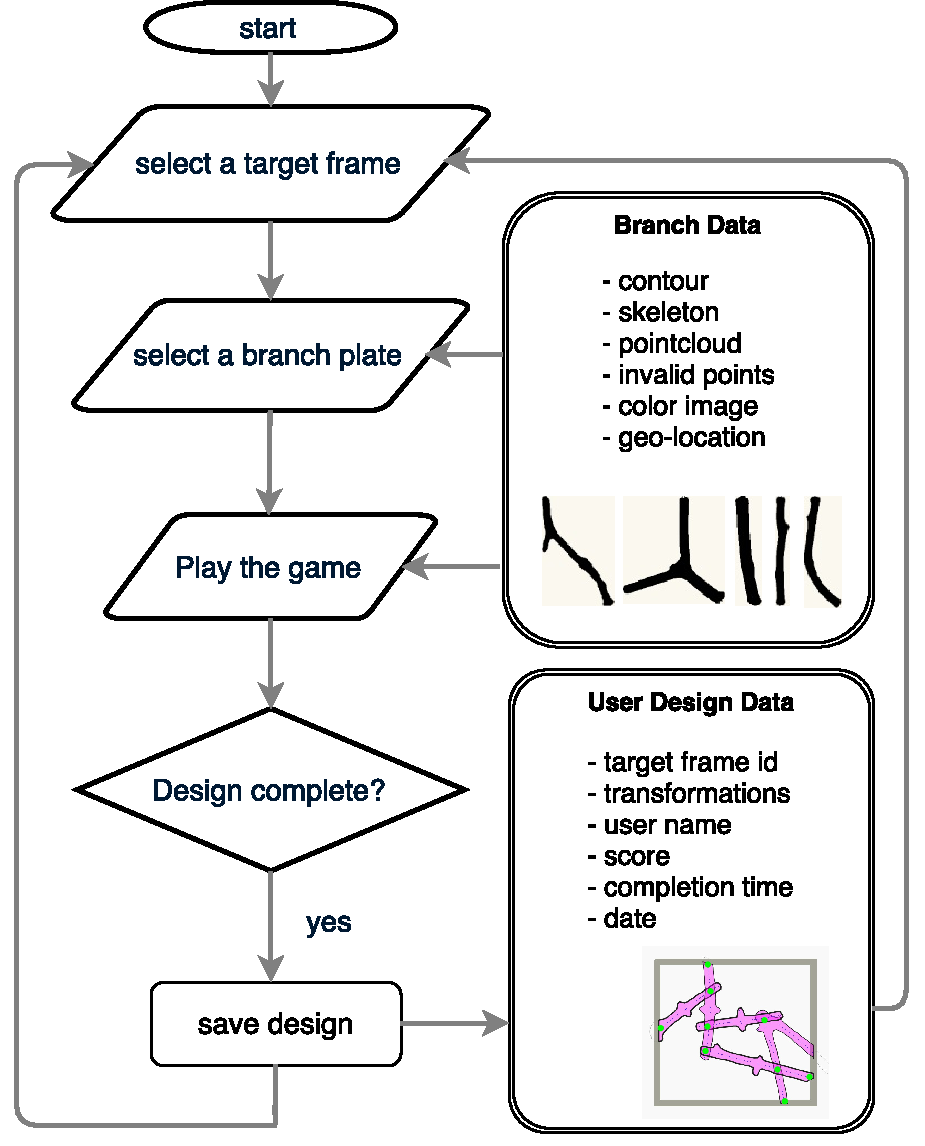
\includegraphics[width = 0.25\paperwidth]{images/system/systemFlowChart.pdf}
%    \caption{The workflow of \textit{BranchConnect}. Branch data and user design data are stored on cloud database.}
%    \label{fig:game_flowchart}
%  \end{center}
%\end{figure}

%Describing user experience, firstly a user selects a target frame indicating multiple target points to be connected, and then selects a set of branches fixed on a plate (the left in Figure \ref{fig:game_interface}).
The overall user experience is as follows.
In the selection interface (Figure \ref{fig:game_interface} left), each frame comes with a set of predefined target points to be connected.
%A user selects a target frame and connect the assigned target points
The distribution of these target points is predefined by the system, and end users can not modify them.
After a user selects a target frame and a set of branches on a plate, the user is guided to the game interface (Figure \ref{fig:game_interface} right), consisting of the frame with the target points, and the set of available branches at the bottom.
The user picks a branch from the available set on the bottom, and drag\&drop it to the inside of the target frame.
By selecting and dragging these dropped branches, the user searches a good 2D pose through basic direct geometric manipulations such as move, rotate, and horizontal flip (or mirror).
While the manipulation, the user receives simple feedback with colors and score.
Within the limited number of available branches, the user needs to bridge all the target points by connecting all the dropped branches in one group.
The game is completed when all the target points are connected.
To achieve higher score, the user can keep modifying the design, and save it to the database.

\begin{figure}[ht]
  \begin{center}
    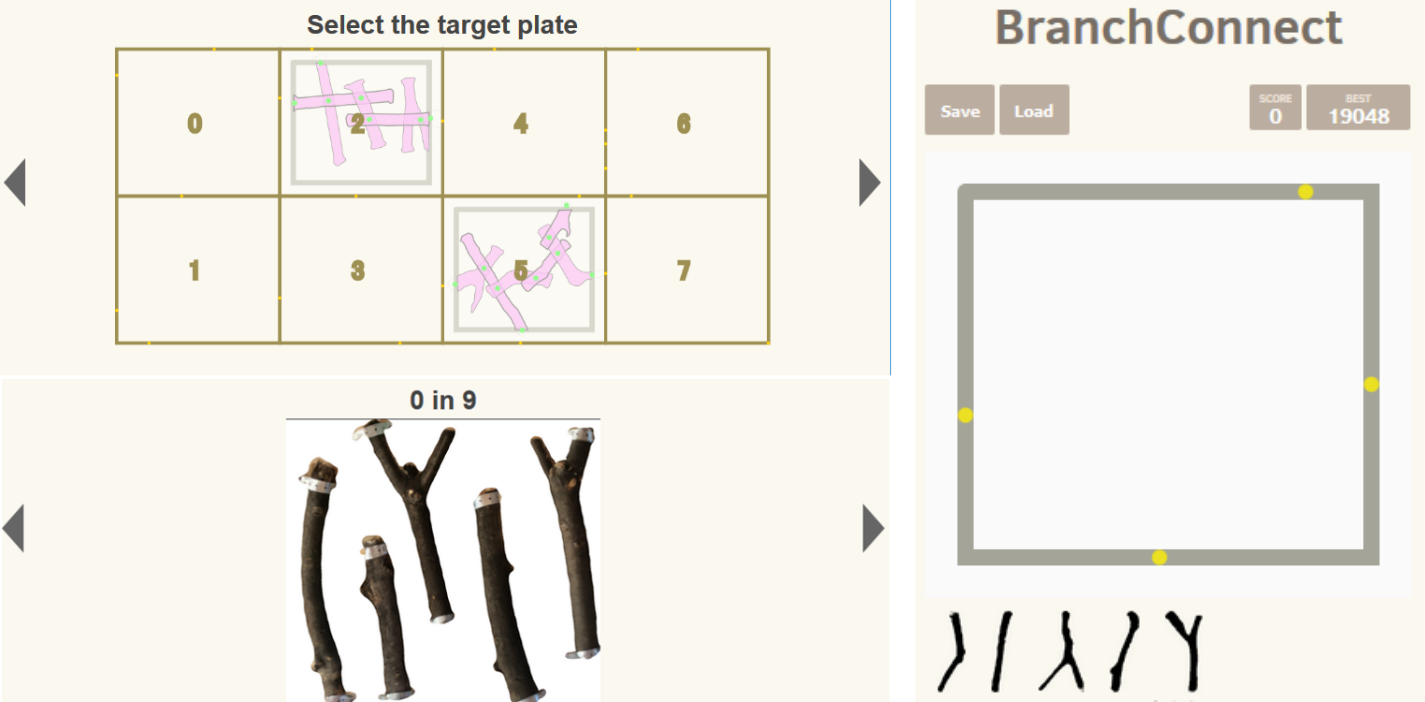
\includegraphics[width = 0.4\paperwidth]{images/interface/game_interface.png}
    \caption{Left: the selection interface for target frames (top) and branch panels (bottom). Right: the start interface of the game.}
    \label{fig:game_interface}
  \end{center}
\end{figure}
%
\subsection{The Game System}
There are many physics simulation libraries for game, however, our game needs to detect intersected branch pairs, thus collision detection with physics engines is overkill for our browser game.
%Our game is running on browsers with rich 
Also, branches have free-form concave shapes, thus further geometric preparation such as convex decomposition is necessary for using these libraries.
For fast and robust intersection detection, our game extensively uses down-sampled skeletons of branches.

Hubbard and Philip developed collision detection by representing an object with hierarchical 3D spheres aligned on a skeleton \cite{Hubbard:1996:APS:231731.231732}.
Our game takes similar approach but limited in 2D, but more focused on searching fabricatable joints.
In the game, down-sampled skeletons are used to find the pair of closest skeleton points between two branches.
While a branch is selected, the system searches the closest skeleton point of the selected branch with other skeletons of available branches.
If the distance of a pair of the closest skeleton points is smaller than a threshold, the pair is intersected.
More precise joint calculation with high-resolution contours is further described in Section \ref{sec:fabrication}.


Here, we introduce two important entities in the game: joint and group.
A joint is created when an intersecting pair is detected, and the pair forms a group.
The group is used for evaluating connections between target points.
The conditions of joint and group are indicated with simple color-code.
Once the user finishes geometric manipulation, score is updated with weighted sum of score parameters.
Together with the color-code, the score update guides the user to form a feasible design.



\subsubsection{Joint Condition}
\label{sec:joint}
Joint is the essential entity not only in the game but also in the fabrication process of customized lapped joints.
Importantly, each pair of branches must have one flipped branch for fabrication constraint (Section \ref{sec:fabrication}).
Figure~\ref{fig:joint_condition} illustrates valid and invalid joint conditions.
Our joint takes only crossed pair because they are structurally stable, relatively simple to fabricate, and creates diverse designs (Figure~\ref{fig:joint_condition}.1). 
Due to fabrication process with CNC milling, we do not take conditions such as terminal connection, joint at metal fixture, and T-shaped connection (Figure~\ref{fig:joint_condition}.3, \ref{fig:joint_condition}.4, and \ref{fig:joint_condition}.5 respectively) .
A valid joint's angle stays within a fixed range (Figure~\ref{fig:joint_condition}.1 and 2).
Valid and invalid joints are displayed with green and red respectively.

\begin{figure}[ht]
	\begin{center}
		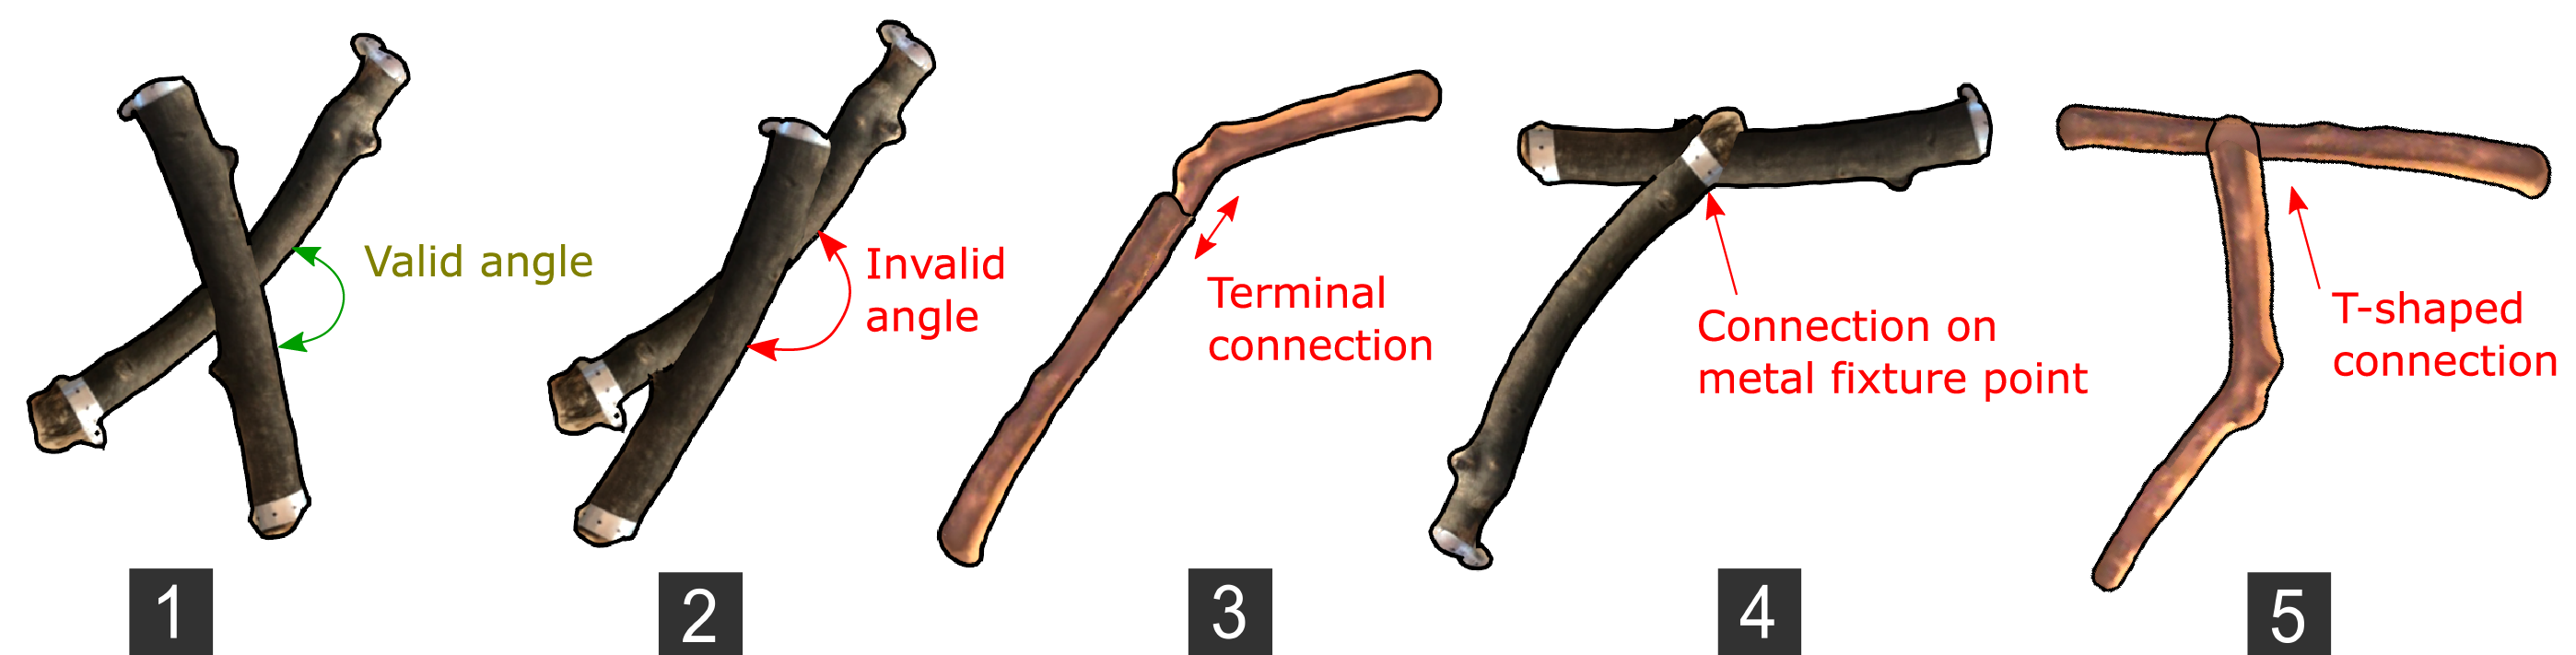
\includegraphics[width = 0.4\paperwidth]{images/system/joint_conditions_3.png}
		\caption{Joint conditions. 1. valid joint. 2. invalid for violating the angle. 3. invalid terminal connection. 4. invalid for connecting on a metal fixture point. 5. invalid for T-shaped connection.}
		\label{fig:joint_condition}
	\end{center}
\end{figure}




To describe the joint update process, let each branch $b_i$ be a member of a set of the branches $\mathcal{B}$ dropped inside of the target frame by a user.
The user freely choose $\mathcal{B} \in \mathcal{B_\text{plate}}$, where $\mathcal{B_\text{plate}}$ is the branches fixed on a selected plate, denoted as $\mathcal{B_\text{plate}}$.
Note that we accept one joint with a pair of branches, but a branch can have multiple joints with other branches. 
The process starts from the selected branch $b_i$ and updates joint conditions of the selected branch with paired branches.
When an intersected pair is detected, it stores $j$-th joint $j_{i, j}$ in $b_i$ with joint conditions (Figure~\ref{fig:joint_condition}).
After evaluation, as in Figure \ref{fig:joint_condition},  we have joints labeled as valid or invalid.
When a branch $b_i$ is connected to one of target points $t_j \in \mathcal{T}$, the target point $t_{i, j}$ is stored in $b_i$.
Note that we also take one target point per branch.
The branch connected to the target point is trimmed at the target point.
The trimmed length $l_{\text{trim}, i}$ is stored in $b_i$ and use as a penalty for score calculation.
In this way, the user tries to position the branch as inside of the frame as possible. 
This process is iteratively executed while a user is positioning a branch while dragging.


%\begin{figure}[h]
%	\begin{center}
%		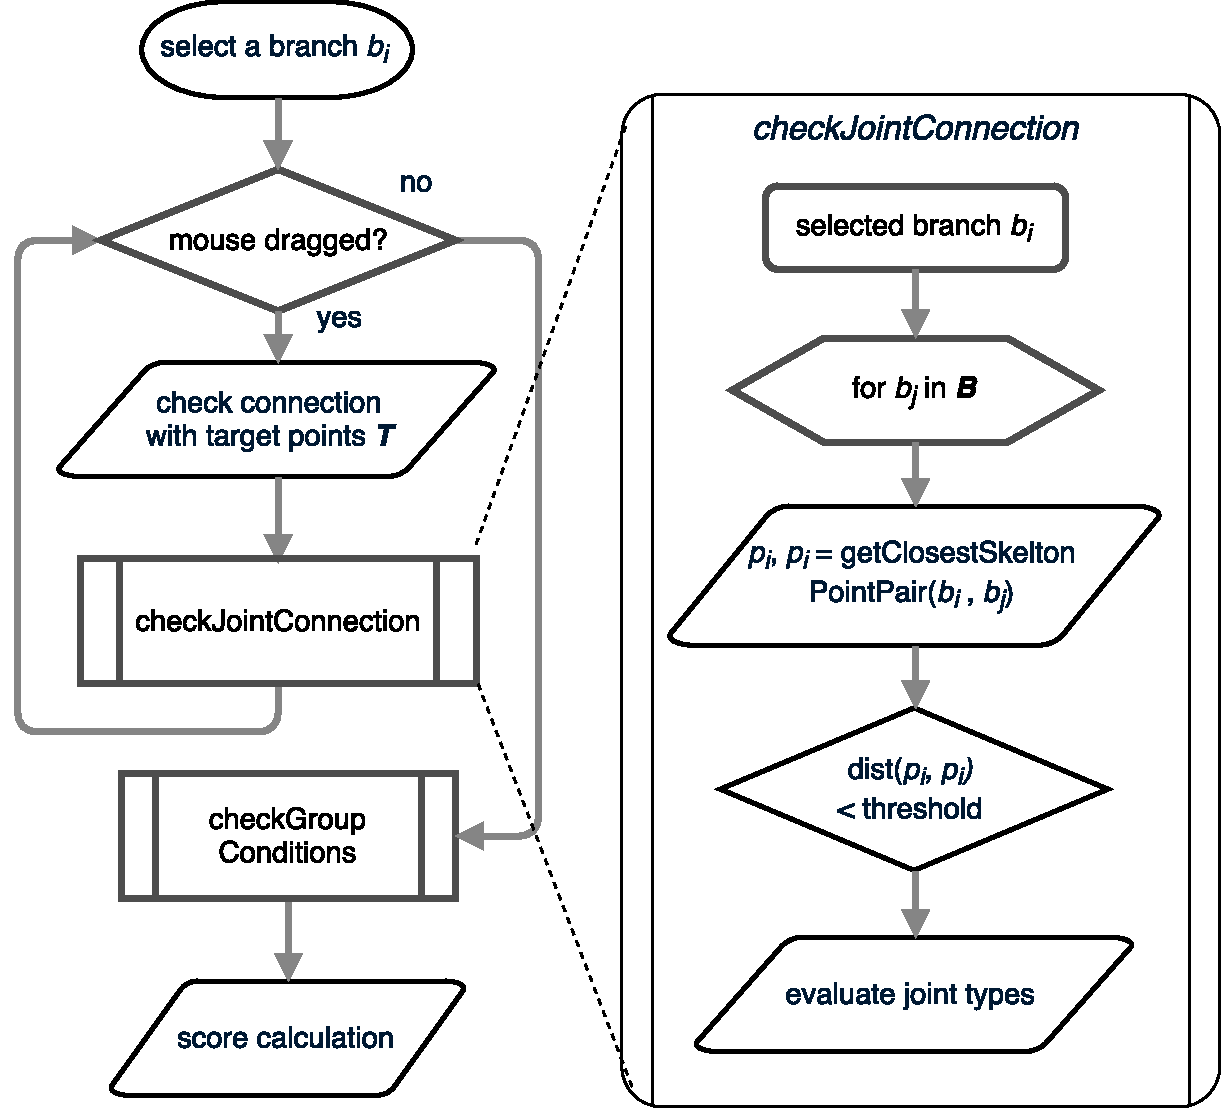
\includegraphics[width = 0.35\paperwidth]{images/system/closestPointAlgorithm.pdf}
%		\caption{Left: an overview of the game system with 1. joint update 2. group update and 3. score calculation. This process is iteratively executed while a user is exploring layout by dragging a branch. The joint update process is further illustrated in the right, and group condition update is described in Algorithm \ref{al:connection}. }
%		\label{fig:system_flowchart}
%	\end{center}
%\end{figure}

% well as the paired branch $b_{\text{paired},j} \in \mathcal{P}_{\text{paired},i}}$.



\subsubsection{Group Condition}

After a user finishes positioning a branch, the system evaluates group conditions.
Firstly it updates groups, and then detects invalid group conditions, as well as connections to target points.
If a branch is connected to a target point, colors of the branch and its belonging group are updated, guiding users the validity of their layouts.
When a group bridges a pair of target points, a special score is added and displayed with an animation.

The group update process is described as follows.
Each time the process is called, firstly it initializes a set of groups denoted as $\mathcal{G}$.
Iterating $b_i \in \mathcal{B}$, the first group $g_0 \in \mathcal{G}$ is created and $g_0$ stores $b_0$.
In the iteration, the process checks connections of a branch $b_i$ with all the existing groups $ g_j \in \mathcal{G}$.
If $b_i$ is connected to $g_j$, $g_j$ is stored in a list of connected groups, denoted as $C_i$.
After collecting all the connected groups with $b_i$, we evaluates $C_i$.
If $C_i$ does not have any stored group, then a new group $g$ storing $b_i$ is created and added to $\mathcal{G}$.
If $C_i$ is not empty, then it also creates a new group $g$, but puts all the groups $g_j \in C_i$ to $g$, then adds $g$ to $\mathcal{G}$.
Finally groups $g_j \in C_i$ are removed from $\mathcal{G}$.
Iterating all $b_i \in \mathcal{B}$, we acquire the updated group condition.

After updating the group, the process evaluates the connections with target points.
If $b_i \in g_k \in \mathcal{G}$ has a connection with a target point, the target point is stored in the group $g_k$.
If multiple groups with target points for each exist, the entire structure is feasible, however, these groups should be connected together (Figure \ref{fig:group} middle).
If the group does not have any target point, the group is labeled as \textit{Islanded}, which is structurally infeasible thus counted as a penalty in the cost calculation (Figure \ref{fig:group} right).
If the group has multiple target points, these target points are bridged.
The game completes when the number of $\mathcal{G}$ is one, and all the target points are connected with the group, which does not have branches with invalid joints.
The group update process is described in Algorithm \ref{al:connection}.
%The entire flowchart of the joint update process as well as the group update process are illustrated in Figure \ref{fig:system_flowchart}.

\begin{figure}[ht]
  \begin{center}
    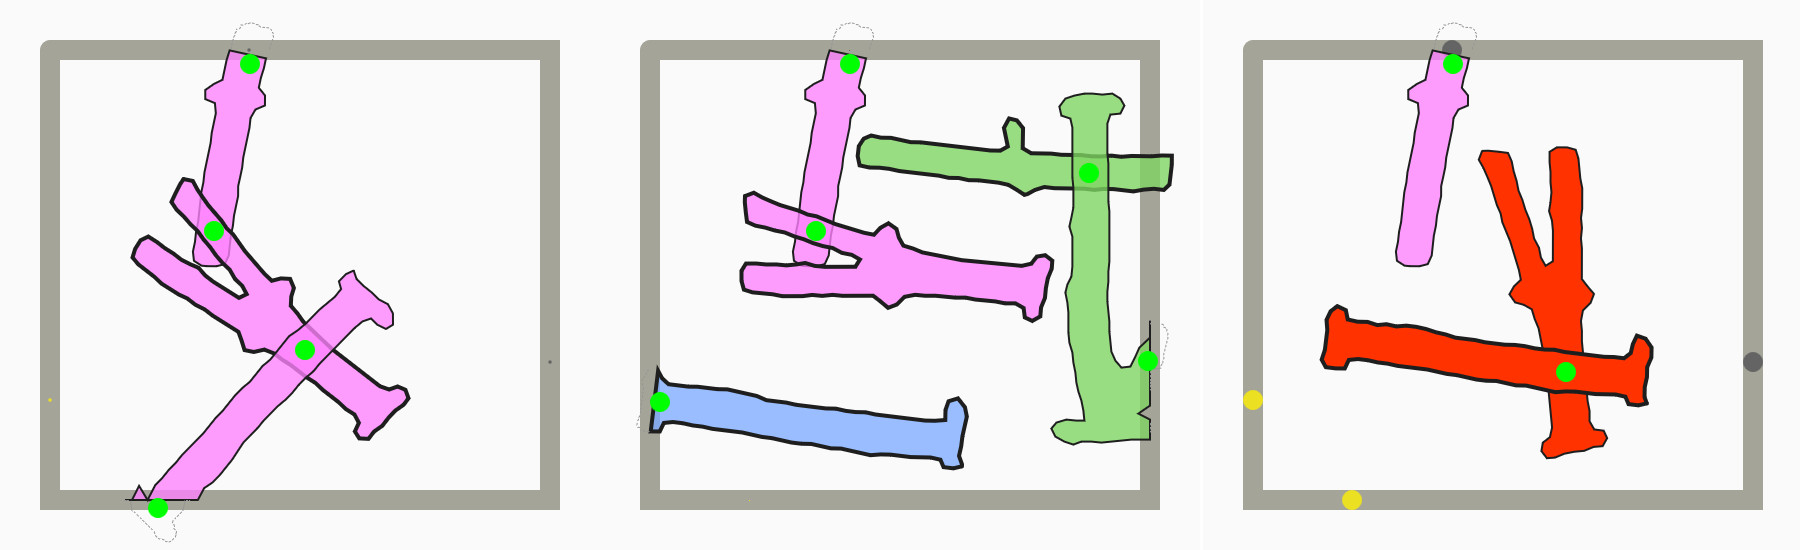
\includegraphics[width = 0.4\paperwidth]{images/interface/groups.jpg}
    \caption{Left: valid group with two target points connected. Middle: valid but three groups. Right: invalid due to the \textit{Islanded} situation. }
    \label{fig:group}
  \end{center}
\end{figure}

\begin{algorithm}
  \caption{Group Condition Update Algorithm}
  \begin{algorithmic}[1]
    \Function{UpdateGroups}{$\mathcal{B}$}
    \State{Reset all the groups $\mathcal{G}$ }
    \State{Create new group $g_0$}
    \State{$g_0$.adds $\left( b_0 \right) $}
%    \If{$b_0$.contains$\left( t_i \in \mathcal{T} \right) $ }
%      \State{$g_0$.adds$\left(t_i \right) $}
%    \EndIf
    \State{$\mathcal{G}$.adds$\left( g_0 \right) $ }

    \For{each branch $b_i \in \mathcal{B}$ except $b_0$}
    \State{\textit{initiate a list of connected group} $C_i$}
      \For{each group $g_j \in \mathcal{G}$}
          \If{ $g_j$.contains$ \left( b_i \right)$}
            \State{ $C_i$.add$\left( g_j \right) $}
          \EndIf
      \EndFor
      
  	\State{Create new group $g$}
	\If{$C_i$.hasMember}
		\For{each group $g_j \in  C_i$}
			\For{each branch $b_k \in g_j$}
%				\If{$g$.contains$\left( b_k \right) =false$}
						\State{$g$.adds$\left(b_k \right) $}
%				\EndIf
			\EndFor
		\EndFor
		\For{each group $g_j \in  C_i$}
			\State{$\mathcal{G}$.removes$\left(g_j \right) $}
		\EndFor

	\EndIf
	\State{$g$.adds$\left(b_i \right) $}
	\State{$\mathcal{G}$.adds$\left( g \right) $ }
	\EndFor
  \EndFunction
  \end{algorithmic}
  \label{al:connection}
\end{algorithm}

\subsubsection{Score Calculation}
We calculate the score with weighted sum of following entities: the numbers of valid and invalid joints on each branch as N($\mathcal{J}_{\text{valid},i}$) and  N($\mathcal{J}_{\text{invalid},i}$) respectively, the number of groups as $N(\mathcal{G} )$, the number of islanded groups as $N(g_{\text{islanded}})$, the number of bridged target points as $N(t_{\text{bridged}, i})$.
The trimmed length $l_{\text{trim}, i}$ in each $b_i \in \mathcal{B}$
The score is weighted sum of these joint and group conditions, denoted in Equation (\ref{eq:score}).
The weights $w_1 \dotso  w_5$ are non-negative weight coefficients pre-adjusted in advance by authors.


\begin{equation} 
 \begin{aligned}
 Score =  &\; w_1\;  \sum_{1}^{N(\mathcal{B})} N(\mathcal{J}_{\text{valid},i})\; +  \;w_2\; \sum_{1}^{N(\mathcal{B})} N(\mathcal{J}_{\text{invalid},i})\\
		+ &\; w_3\;  N(g_{\text{islanded}} \in \mathcal{G} )\;				 	 \;+  \;w_4\;  N(t_{\text{bridged}, i}) \; +  \;w_5\; \sum_{1}^{N(\mathcal{B})} l_{\text{trim}, i}
 \\
   \textrm{s.t.} \; w_j  \geq  &\;0 \; \forall j \in 1, \dotsc , 5 
 \end{aligned}
 \label{eq:score}
\end{equation}

\section{Case Study}
\label{sec:casestudy}
A design and fabrication workshop was organized to examine the feasibility of our system with a specific design target and a location.
We selected a public community house where people in the community share the space and regularly use the facility.
Participants of the workshop were selected among them, who were four children (aged 4, 7, 9, and 10) and two parents (Figure~\ref{fig:workshop}).
We specifically selected children with this range of age as non-experts without experiences in computational design or digital fabrication, also for observing the clarity and attractiveness of the game.
The entire workshop was filmed and documented in a short clip.
Please refer the supplementary video material for the documentation.

The goal for the participants was to contribute to an ongoing design and fabrication process of screen wall (2000 $mm$ $\times$ 900 $mm$) consisting of eight rectangles (500 $mm$ $\times$ 450 $mm$).
Six frames were already designed and built, thus the rest two frames were prioritized for them to design and fabricate in this workshop.

Participants were informed about the goal of the workshop, and each process was introduced by experienced tutors.
The processes were from collecting and fixing the branches on a plate, scanning the plate, complete designs by playing the game, and assembly after CNC milling.

\begin{figure}[ht]
  \begin{center}
    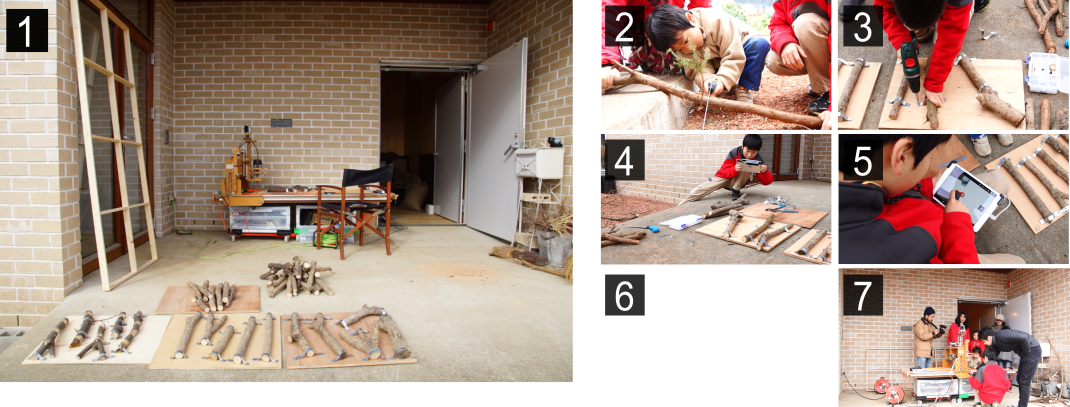
\includegraphics[width = 0.4\paperwidth]{images/fabrication/workshop_setup.png}
    \caption{An overview of the workshop. 1. the overview of the space. 2. collect branches. 3. cut in certain lengths 4. attach on a plate 5. scan the plate 6. play the game 7. CNC milling.}
    \label{fig:workshop}
  \end{center}
\end{figure}

\subsection{Preparations and User Experiences}
\subsubsection*{System and Hardware}
We used two iPad minis with iSense depth cameras attached for scanning branches, and a 3 axis CNC milling router with a 6 mm diameter milling bit.
We used a laptop PC for running \textit{Branch Importer} and \textit{G-Code generator}, as well as operating the milling machine.
The scan area of iSense camera is 500 $mm$ $\times$ 500 $mm$, and the milling machine's stroke length along z-axis is 70 $mm$, which provide geometric constraints for available branch sizes.
\textit{BranchConnect} was hosted at \textit{Heroku} cloud server \footnote{ Heroku is a platform as a service (PaaS) that enables developers to build, run, and operate applications entirely in the cloud. \url{https://www.heroku.com/}},
and we used \textit{MongoDB} \footnote{ MongoDB is a free and open-source cross-platform document-oriented database program. \url{https://www.mongodb.com/}} as a cloud database.

\subsubsection*{Preparations}
The participants were asked to collect branches with 20 - 100 $mm$ in diameter.
The lower bound of the diameter was set due to the milling bit size, and the upper bound was set for the limited length of z-stroke of the CNC router.
The collected branches were cut in arbitrary lengths, not longer than 500 $mm$ due to the limit of scanning area. 
As our game system and fabrication process take 3D branch shapes as 2D contours (with limited use of point cloud), these constraints worked positive for the system by filtering out branches with large 3D twists.
The diameter and length constraints worked as guidelines for participants rather than restricting finding and cutting arbitrary branches.

After cutting branches in certain lengths, participants fixed branches on plates by thin metal plates with screw holes.
It was straightforward for them to firmly fix branches so that they are not moved during milling process.
%These fixture points are counted as invalid points in the game where joinery points can not be generated.
The participants built two plates with three and five branches fixed on each plate.

After finidhing the plates, we asked participants to scan with iPad + iSense and prepare feasible mesh model by themselves.
Thanks to the intuitive interface of iSense, participants practiced several scans and successfully scanned models without problem.
After obtaining mesh models, tutors imported models from iPads to a laptop and upload them to database by \textit{Branch Importer}.



\subsubsection*{User Experiences}
%After models were uploaded to the server, participants could that their plates are added in the selectable branch plates with their names and locations.
As for more general user experiences with the game, see Section \ref{sec:game} as well as the video material.
%Users could access to the start page by PC and mobile devices.
In this section, we describe more specific user experiences and feedback from participants.

%We prepared both options and let participants choose a device.
All participants used iPads for navigating pages and playing the game.
They had difficulties with mobile touch interface, such as rotation and flipping operation by gestures.
We had several requests from participants regarding the game interface but also related to the workshop organization. Several participants requested to allow multiple branch plates for designing a frame, or even remove the target frame and let them freely design with branches.
Also a participant who gave up the game with iPad requested additional buttons for mobile touch interface, such as to keep an active branch selected.
The participant with four years old failed to complete the game.
He insisted on accepting his design to be fabricated 
Similarly, a branch plate made by a participant had only three branches, which was not enough to fulfill bridging target points, however, the participant insisted on accepting it in the selection.
%We took them as positive inputs to validate our participatory (architectural) design approach.
%A user is firstly directed to a start page and asked to submit a user name.
%Secondly, the user is navigated to target frame selection page, and asked to pick one out of eight frames.
%Each frame has different target points.
%The interface also shows the completed branch organizations within each target frame.
%If there are multiple designs, three designs with highest scores are displayed.
%The user can change the currently displayed design by clicking within each frame and choose either starting their design from scratch, or select the design and improve it.
%After selecting a target frame, the user goes to branch selection page, displaying 15 plates when the workshop was held.
%In this page, they saw the plates made by themselves on the page, as well as their names on the plate.
%The user can select the same plate for designing other target frames.
%By clicking a displayed branch plate, the user is navigated to the game interface.
%After completing to bridge all the target points, the design is automatically uploaded to the database, but the use can continue to design.


\subsubsection*{Global Design Consensus and Fabrication} 
As the target frame selection page could display all layout designs, we could get an overview of design options.
The layout designs were displayed as score descending order with limited numbers (three top highest scores for each target frame), we could find feasible layout designs easily with mostly all the target points were bridged.
As participants were excited by seeing their branches and designs, we took two invalid layout designs and one plate which did not have enough branches for the global design.
%
%\subsubsection*{Fabrication}
After selecting layouts, an experienced tutor operates \textit{G-Code Generator} as well as the CNC router.
Participants were asked to assembly branches after joineries were milled.

\subsection{Results}
The entire workshop took 4.6 hours to complete the whole process, including introduction, moving, and pauses.
Table \ref{tab:timing} shows durations of each task.

\begin{center}
  \begin{tabulary}{\columnwidth}{ |l||C|C| }
    \hline
    Task & Duration (hour) & Fraction ($\%$) \\
    \hline
    Introduction                  & 0.3 & 6.5  \\
    Collecting branches           & 0.6 & 13.0  \\
    Preparing plates              & 0.8 & 17.4  \\
    Preparing models              & 0.3 & 6.5  \\
    Uploading models              & 0.2 & 4.3 \\
    Designing by the game         & 0.5 & 10.8 \\
    Inspecting models             & 0.2 & 4.3 \\
    CNC milling                   & 0.5 & 10.8\\
    Assembling                    & 0.2 & 4.3 \\
    Moving, pauses               & 1.0 & 21.7 \\
    \hline
    In total                      & 4.6   & 100 \\
    \hline
  \end{tabulary}
  \label{tab:timing}
\end{center}



\subsubsection*{Model Acquisition}
Each scanning and re-touching took 2-3 minutes, and 30 seconds for generating data by \textit{Branch Importer}.
Including the prepared panels previously, we scanned 15 plates in total, 75 branches, and 35.3m of total length including sub-branches.
We got 59 branches with a single skeleton, 16 branches with multiple skeletons for grafting.
The result is shown in Figure \ref{fig:scannedplates}.

\begin{figure}[ht]
  \begin{center}
    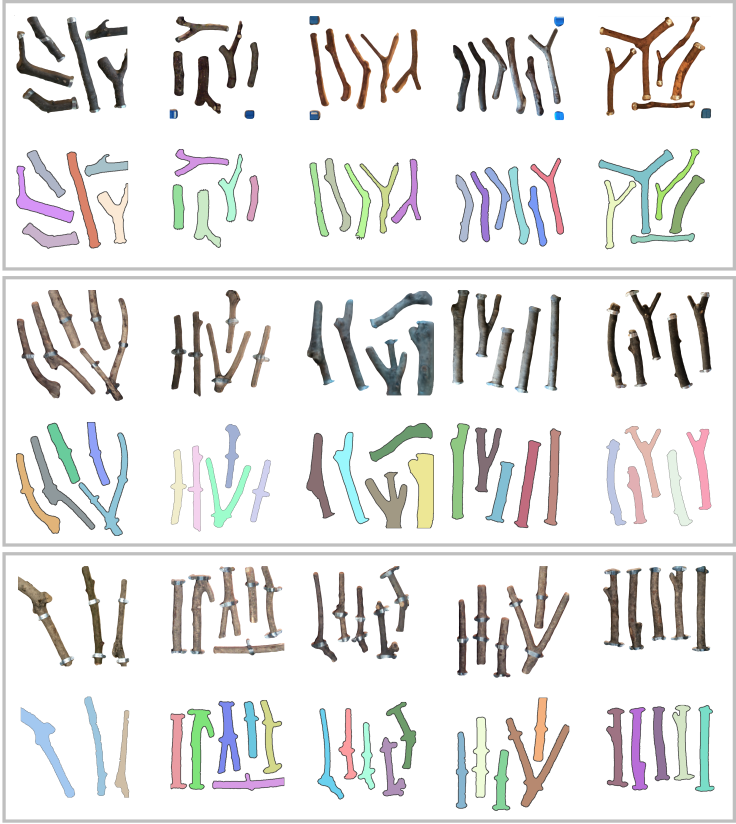
\includegraphics[width = 0.4\paperwidth]{images/fabrication/all_plates.png}
    \caption{An overview of all the 15 scanned plates for the construction of the fence. Top raw of each set shows ortho-top views of scanned mesh models, and the bottom raw is the recognized branches with randomly assigned colors. The red-lined rectangles indicate the plates built by participants in the workshop.}
    \label{fig:scannedplates}
  \end{center}
\end{figure}


\subsubsection*{Design with the Game}


One participant switched to play by a PC for more precise control due to the problem.
Interestingly, all the participants chose to develop their own designs from the scratch, although they had instruction about the "continue existing designs".

We set 30 minutes for playing the game, and eight layout designs were given by participants.
Two frames were completed per participants and two participants completed the whole eight target frames.
The average score was xxx, and average playing duration was xxx to complete each target frame. \todo{recheck the numbers by server}


\subsubsection*{Fabrication}
%We did not have major problems for converting designs to G-Code milling paths as we encountered major issues regarding the fabrication before the workshop, which are reported in this section.

%We encountered problem was the accuracy of acquired contours.
We observed most of scanned models had occluded regions between plates and branches, which create interpolated faces during solidifying process, resulting in outwardly offsetted contours. \todo{check offsetted correct english} After milling was finished and when branches were assembled, six pairs of branches were loosely connected because the calculated contours were 2-3 $mm$ eroded than the actual sizes.
We avoided this problem by trimming branches from 2-5 $mm$ higher than the plate surface.
After this operation, the rest of connections were tightly connected. \\

We also observed that many milling paths were 5-10 $mm$ off from the center of planned joints.
Multiple reasons could be considered as reasons such as,

\begin{itemize}
  \item{deformation of mechanical parts of the CNC router}
  \item{not dense resolution of acquired contours of branches}
  \item{misaligned orientation of the plate compared to the scanned model}
\end{itemize}

To avoid the misalignments, we modified the \textit{G-Code Generator} so that an operator can freely adjust the absolute origin of the generated milling paths.
The origin was usually set with around the center of the plate.
After this modification, the misalignment from joint center was reduced with 5 $mm$ off at the maximum misalignment.
Branches could absorb 3-5 $mm$ misaligned joint positions due to the elasticity of branches, and solidifying the structure with residual stresses from misalignments.
% The misaligned joint positions worked as post-tensions, solidifying the structure.
% We assume that this is only applicable when an applied bending moment and cut surface at a joint is orthogonal or not too much off from orthogonal. \todo{this sentence}





\section{Conclusion}
% \subsubsection*{Summary}
In this paper, we presented a workflow to design and fabricate with branches with their native forms, which are not large enough for producing standardized building components.
Our workflow was validated by the case study with lower-aged participants without design and fabrication experiences.
Our online platform with stored scanned branches is accessible and multiple users can submit design layouts and explore a global design. % and locations.
Our branch joint detection and group condition update algorithms are running on the browser game which can be accessed from laptops and mobile devices, contributing to the accessibility of the presented workflow.
Together with the accessibility, the intuitive interface was simple for non-expert users, validated by the case study.
We successfully built a network of branches with rigid joints generated by our joinery milling path generator.
Each of joints has customized lapped-joint geometry, which extends design possibilities of branches or woods with their native forms.

% \subsubsection*{Limitations and Future Work}
Our workflow touches many developed research areas such as skeleton extraction, structural optimization, object detection/recognition, and data-driven design-fabrication.
Focusing on the use of native forms, each step of our workflow has potential to contribute to each area with the use of native forms of natural materials.
Also, our workflow was developed based on the participation of users, thus the entire process is not necessarily automated, however, some tasks could be improved to assist users.\\

The skeleton extraction could take incomplete point-set directly from original tree branches before they are cut in length.
With data-driven approach, the system could distinguish trees and which part of tree the branch from.
With morphological analysis, the system could suggest users where to cut branches to achieve user-defined target design.
Structural and geometrical validity/invalidity of obtained materials could be analyzed.
Our workflow requires branches to be fixed on a plate, which takes the longest duration in the workflow except for in-between tasks such as moving and pausing.
Using a robotic manipulator with a gripper, the attaching process could be skipped.

Our game system is limited in 2D, whereas original branch forms have rich 3D geometry with textures.
In our case, these information was used in limited ways such as in skeleton extractions and G-Code generation.
Despite of successfully fabricated non-orthogonal joineries, we did not complete the attaching branches to the target frames, as we prioritized to validate branch-branch joineries.
Our layout design process is fully dependent on users with limited feedback during design process.
The game can provide suggestive feedback with structural analysis of each joint and entire structure.
% As the problem of limited number of branches and fixed target points to be connected, the system could assist humans to reach to structurally sound solutions with less efforts.

% The performance of our joint detection and alalgorithm could be
Our joint and group detection algorithms are limited with materials with skeletons, and our joinery generator is limited to branches.
Both steps use down-sampled or high-resolution point sets.
It is valuable to validate the approach by comparing with other available methods such as collision detections or joint detection with down-sampled model by interpolation.

Finally, our game-based design could be applied to different purposes, not only for participatory layout design but also for collecting data of user behaviors during design.
Also application to other kinds of materials could be investigated.



%\section*{Acknowledgments}
%We appreciate the public house for hosting the CNC router and providing participants for the user study.
%We thank to the film editor, Shin Yamane for shooting our video clips.
%We also thank to the developer of an online game \textit{2048}, Gabriele Cirulli and his contributors, for sharing source code in Github community.


\bibliographystyle{acmsiggraph}
\nocite{*}
\bibliography{references}
\end{document}
